% Input common header
\documentclass[xcolor=dvipsnames]{beamer}

\usecolortheme[named=Blue]{structure}
\setbeamertemplate{itemize items}[circle]

\usepackage{smartdiagram}


\author{Dr. Paul Larsen}
\date{\today}



\title{Discrete Geometry for Risk and AI}
\begin{document}
\maketitle

\begin{frame}
\frametitle{Why discrete geometry?}

\begin{itemize}
\item Older history: graphical models among first non-rules based AI approaches \cite{darwiche2009modeling}
\item Recent history: Dissatisfaction with deep learning, only ``curve fitting'', alternative via \emph{causal graphical models} \cite{pearl2019limitations}
\item Geometrical formulations of statistical objects, e.g. graphical models and probability polytopes\newline
\end{itemize}

\end{frame}

\begin{frame}
  \frametitle{Directed graphical model: university admission gender bias}
  \framesubtitle{Simpson paradox preview}

  \begin{figure}[ht]
    \centering
            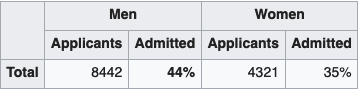
\includegraphics[height=0.15\textwidth]{graphics/berkeley} 
            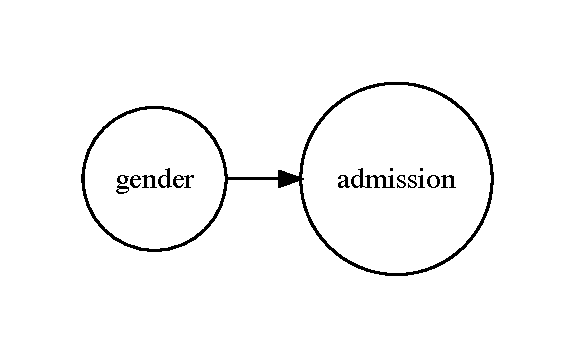
\includegraphics[height=0.4\textwidth]{graphics/admission_original}
       
    \end{figure}
    Sources: \cite{simpson-wikipedia} \cite{freedman1998statistics}
\end{frame}

\begin{frame}
  \frametitle{Bayesian networks: university admission gender bias}
  \framesubtitle{Simpson paradox preview}

  \begin{figure}[ht]
    \centering
            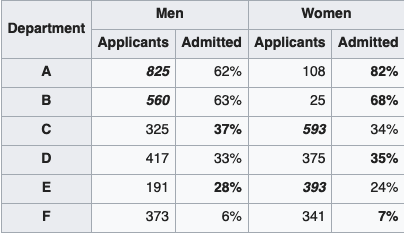
\includegraphics[height=0.35\textheight]{graphics/berkeley_later} 
            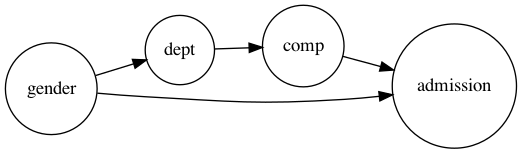
\includegraphics[height=0.35\textheight]{graphics/admission_later}
    \end{figure}
    Sources: \cite{simpson-wikipedia} \cite{Bickel398}
\end{frame}

\begin{frame}
\frametitle{Directed graphical model: hit rate for insurance quotes}
\begin{itemize}
  \item product type: financial, liability, property
  \item days: number of days to generate quote
  \item rating: measure of premium paid expected claims
  \item hit: 0 if quote refused, 1 if accepted
\end{itemize}
\begin{figure}[ht]
  \centering
  \includegraphics[height=0.7\textheight]{graphics/hit}
\end{figure}
\end{frame}


\begin{frame}
\frametitle{Undirected graphical model: credit default risk}

\begin{itemize}
  \item Nodes take values 0 (healthy) or 1 (default)
  \item Industry nodes connect to other industry nodes
  \item Individual firm nodes connect only to corresponding industry node
\end{itemize}
\begin{figure}[ht]
  \centering
  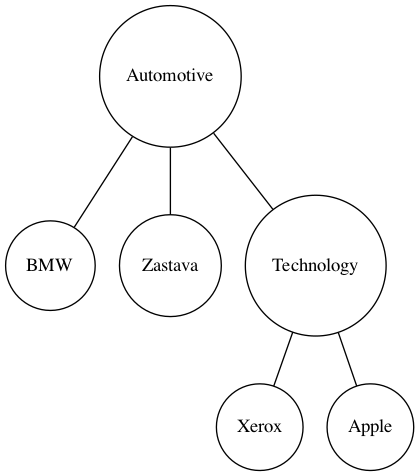
\includegraphics[height=0.7\textheight]{graphics/credit_default}
\end{figure}
\end{frame}


\begin{frame}
\frametitle{Graph definitions}
\begin{definition}
A \emph{graph} is a pair of sets $(V, E)$, where $V$ is called the set of \emph{vertices} (or \emph{nodes}) and $E$ is called the set of \emph{edges}, such that the set of edges corresponds injectively to pairs of vertices. \newline
\end{definition}

\emph{Notes}
\begin{itemize}
\item Typically `pairs of vertices` does not include self-pairs, but this can be relaxed, leading to graphics with with loops.
\item The injectivity requirement can also be relaxed, leading to \emph{multigraphs}.
\end{itemize}
\end{frame}


\begin{frame}
\frametitle{Graphical models}
\begin{definition}
(Informal) A graphical model is a graph whose nodes represent variables and edges represent direct statistical dependencies between the variables.\newline
\end{definition}

\emph{Why graphical models?}
\begin{itemize}
\item For probability distributions admitting a graphical model representation, then graph properties (\emph{d-separation}) imply conditional independence relations.
\item Conditional independence relations reduce the number of parameters required to specify a probability distribution.
\item Graphical models come in two flavors depending on their edges: directed (aka \emph{Bayesian Networks}) and undirected (aka \emph{random Markov fields}.
\end{itemize}
\end{frame}




\begin{frame}
\frametitle{d-separation in DAGs}
\begin{definition}
Let $X$, $Y$, and $Z$ be three disjoint subsets of nodes in a directed acyclic graph, $G$, and let $p$ be any path between a node in $X$ and one in $Y$, where by `path'we mean a succession of arcs, independent of direction. Then $Z$ is said to block $p$ if there is a node $w$ on $p$ satisfying one of the following two conditions

\begin{enumerate}
\item $w$ has converging arrows along $p$, and neither $w$ nor any of its descendents are in $Z$, or
\item $w$ does not have converging arrows along $p$, and $w$ is in $Z$.
\end{enumerate}

Further, $Z$ is said to $d-separate$ $X$ from $Y$ in $G$, denoted 

\begin{equation*}
    (X \ci Y | Z)_G
\end{equation*}

if and only if $Z$ blocks every path from a node in $X$ to a node in $Y$.\newline
\end{definition}
References: \cite{pearl1995causal}
\end{frame}


\begin{frame}
\frametitle{d-separation}
\framesubtitle{Intuition}
From \cite{scheines-tutorial}: \newline

\begin{quote}
Roughly, two variables $X$ and $Y$ are independent conditional on $Z$ if knowledge of $X$ gives you no extra information about $Y$ once you have knowledge about $Z$. In other words, once you know $Z$, $X$ adds nothing to what you know about $Y$.
\end{quote}

\end{frame}

\begin{frame}
    \frametitle{d-separation}
    \framesubtitle{Alternative definition via blocking paths}
    
 
\end{frame}

\begin{frame}
    \frametitle{d-separation}
    \framesubtitle{Alternative definition, ii}

    Let $A$, $B$, $C$ be non-intersecting subsets of vertices of a DAG $G$. \newline

    \emph{Definition} A path from $A$ to $B$ is \emph{blocked} by $C$ if the path contains a node such that either

    \begin{itemize}
    \item the node is in $C$, and the arrows on the path at the node meet either head-to-tail or tail-to-tail, or
    \item neither the node nor its descendents is in $C$, and the arrows on the path at the node meet head-to-head \newline
    \end{itemize}

    \emph{Definition} A is said to be $d-separated$ from $B$ by $C$ if all paths from $A$ to $B$ are blocked by $C$. We write

    \begin{equation*}
        (A \ci B | C)
    \end{equation*}

    References: \cite{tum-graphical}

    
\end{frame}


\begin{frame}
    \frametitle{d-separation}
    \framesubtitle{Examples}

    \begin{figure}[ht]
        \begin{center}
          \begin{tabular}{cc}
            \onslide<2->{$(A \ci B | \, \{c\})$}
            \begin{tikzpicture}
                                % Define nodes
                \node[obs]                               (c) {$c$};
                \node[obs, above=of c, xshift=-1.2cm] (a) {$a$};
                \node[obs, above=of c, xshift=1.2cm]  (b) {$b$};
        
                \edge {a} {c} ; %
                \edge {c} {b} ;
              
              \end{tikzpicture} &
              \onslide<2->{$(A \ci B | \, \{c\})$}
              \begin{tikzpicture}

                % Define nodes
                \node[obs]                               (c) {$c$};
                \node[obs, above=of c, xshift=-1.2cm] (a) {$a$};
                \node[obs, above=of c, xshift=1.2cm]  (b) {$b$};
        
                \edge {b} {c} ; %
                \edge {c} {a} ; %
              
              \end{tikzpicture}
          \end{tabular}
          \begin{tabular}{cc}
            \onslide<2->{$(A \ci B | \, \{c\}))$}
            \begin{tikzpicture}
                                % Define nodes
                \node[obs]                               (c) {$c$};
                \node[obs, above=of c, xshift=-1.2cm] (a) {$a$};
                \node[obs, above=of c, xshift=1.2cm]  (b) {$b$};
        
                \edge {c} {a} ; %
                \edge {c} {b} ;
              
              \end{tikzpicture} &
              \onslide<2->{$(A \ci B | \,\emptyset)$}
              \begin{tikzpicture}

                % Define nodes
                \node[obs]                               (c) {$c$};
                \node[obs, above=of c, xshift=-1.2cm] (a) {$a$};
                \node[obs, above=of c, xshift=1.2cm]  (b) {$b$};
        
                \edge {a} {c} ; %
                \edge {b} {c} ; %
              
              \end{tikzpicture}
          \end{tabular}
        \end{center}
        \caption{Examples $A = \{a\}$, $B = \{ b\}$.}
      \end{figure}

\end{frame}

\begin{frame}
    \frametitle{d-separation}
    \framesubtitle{More examples}

    \begin{figure}[ht]
        \begin{center}
          \begin{tabular}{cc}
            \onslide<2->{$\neg (A \ci B | \, \{c\})$, but $(A \ci B | \, \emptyset)$}
            \begin{tikzpicture}
                                % Define nodes
                \node[obs]                               (d) {$d$};
                \node[obs, left=of d, xshift=-1.2cm] (a) {$a$};
                \node[obs, right=of d, xshift=1.2cm]  (b) {$b$};
                \node[obs, below=of d]                (c) {$c$};
                \edge {a} {d} ; %
                \edge {b} {d} ;
                \edge {c} {a} ;
                \edge {c} {b} ;
              
              \end{tikzpicture} &
              
        %       \onslide<2->{$(A \ci B | \, \{c\})$}
        %       \begin{tikzpicture}

        %         % Define nodes
        %         \node[obs]                               (c) {$c$};
        %         \node[obs, above=of c, xshift=-1.2cm] (a) {$a$};
        %         \node[obs, above=of c, xshift=1.2cm]  (b) {$b$};
        
        %         \edge {b} {c} ; %
        %         \edge {c} {a} ; %
              
        %       \end{tikzpicture}
        %   \end{tabular}
        %   \begin{tabular}{cc}
        %     \onslide<2->{$(A \ci B | \, \{c\}))$}
        %     \begin{tikzpicture}
        %                         % Define nodes
        %         \node[obs]                               (c) {$c$};
        %         \node[obs, above=of c, xshift=-1.2cm] (a) {$a$};
        %         \node[obs, above=of c, xshift=1.2cm]  (b) {$b$};
        
        %         \edge {c} {a} ; %
        %         \edge {c} {b} ;
              
        %       \end{tikzpicture} &
        %       \onslide<2->{$(A \ci B | \,\emptyset)$}
        %       \begin{tikzpicture}

        %         % Define nodes
        %         \node[obs]                               (c) {$c$};
        %         \node[obs, above=of c, xshift=-1.2cm] (a) {$a$};
        %         \node[obs, above=of c, xshift=1.2cm]  (b) {$b$};
        
        %         \edge {a} {c} ; %
        %         \edge {b} {c} ; %
              
        %      \end{tikzpicture}
          \end{tabular}
        \end{center}
        \caption{Examples $A = \{a\}$, $B = \{ b\}$.}
      \end{figure}

\end{frame}

\begin{frame}
\frametitle{Probability polytopes}
\end{frame}

\begin{frame}[allowframebreaks]
    \frametitle{References}
    \bibliographystyle{amsalpha}
    \bibliography{../../references.bib}
\end{frame}

\end{document}